\documentclass[letterpaper, onecolumn, draftclsnofoot, 10pt, compsoc]{IEEEtran}
\usepackage{graphicx}
\usepackage[hyphens]{url}
\usepackage{setspace}

\usepackage{geometry}
\geometry{textheight=9.5in, textwidth=7in}

% 1. Fill in these details
\def \CapstoneTeamName{			The Polycules}
\def \CapstoneTeamNumber{		63}
\def \GroupMemberOne{			Joshua Lioy}
\def \GroupMemberTwo{			Corynna Park}
\def \GroupMemberThree{			Jackson Wells}
\def \CapstoneProjectName{		Molecules in 3D?! And in color!? That I can hold in my hand? No way!!!}
\def \CapstoneSponsorCompany{	Oregon State University College of Science Department of Biochemistry and Biophysics}
\def \CapstoneSponsorPerson{	Dr. Victor Hsu}

% 2. Uncomment the appropriate line below so that the document type works
\def \DocType{	%Problem Statement
				Requirements Document
				%Technology Review
				%Design Document
				%Progress Report
				}
			
\newcommand{\NameSigPair}[1]{\par
\makebox[2.75in][r]{#1} \hfil 	\makebox[3.25in]{\makebox[2.25in]{\hrulefill} \hfill		\makebox[.75in]{\hrulefill}}
\par\vspace{-12pt} \textit{\tiny\noindent
\makebox[2.75in]{} \hfil		\makebox[3.25in]{\makebox[2.25in][r]{Signature} \hfill	\makebox[.75in][r]{Date}}}}
% 3. If the document is not to be signed, uncomment the RENEWcommand below
%\renewcommand{\NameSigPair}[1]{#1}

%%%%%%%%%%%%%%%%%%%%%%%%%%%%%%%%%%%%%%%
\begin{document}
\begin{titlepage}
    \pagenumbering{gobble}
    \begin{singlespace}
    	
\includegraphics[height=4cm]{coe_v_spot1}
        \hfill 
        % 4. If you have a logo, use this includegraphics command to put it on the coversheet.
        %\includegraphics[height=4cm]{CompanyLogo}   
        \par\vspace{.2in}
        \centering
        \scshape{
            \huge CS Capstone \DocType \par
            {\large\today}\par
            \vspace{.5in}
            \textbf{\Huge\CapstoneProjectName}\par
            \vfill
            {\large Prepared for}\par
            \Huge \CapstoneSponsorCompany\par
            \vspace{5pt}
            {\Large\NameSigPair{\CapstoneSponsorPerson}\par}
            {\large Prepared by }\par
            Group\CapstoneTeamNumber\par
            % 5. comment out the line below this one if you do not wish to name your team
            \CapstoneTeamName\par 
            \vspace{5pt}
            {\Large
                \NameSigPair{\GroupMemberOne}\par
                \NameSigPair{\GroupMemberTwo}\par
                \NameSigPair{\GroupMemberThree}\par
            }
            \vspace{20pt}
        }
        \begin{abstract}
        	This document covers the Software Requirements Specification for the polychromatic molecules project. The document follows the IEEE Std 830-1998 format and is intended to provide a detailed overview of our project requirements. Content includes the purpose and scope of the project, details regarding required resources, and the specific product requirements.     
        \end{abstract}     
    \end{singlespace}
\end{titlepage}
\newpage
\pagenumbering{arabic}
\tableofcontents
% 7. uncomment this (if applicable). Consider adding a page break.
%\listoffigures
%\listoftables
\clearpage

% 8. now you write!
\section{Introduction}

\subsection{Purpose} %Jackson
This document is intended to give a detailed overview of the requirements of our polychromatic 3D printing project.
Contained in this document will be the information required for an individual to gauge the completeness of our project.
Individuals looking to reproduce the project will be able to use this document to verify that they created an identical product.
Audiences concerned with this document include owners of multi-filament interfaces and single extruder printers, or anyone with access to these tools, and anyone with an interest in creating polychromatic 3D objects.

\subsection{Scope} %Josh
Upon completion of our polychromatic 3D printing project we will have produced a polychromatic 3D printing workflow that is comprised of various open-source and proprietary components. 
This workflow will allow a user who has basic knowledge of 3D printing to print a polychromatic object just as easily as a monochromatic object. 
The workflow will be able to take monochromatic 3D object files, and convert them into polychromatic 3D object files that can be printed with the appropriate hardware.\par
Initially we hope that the workflow will allow for faculty and staff in the Oregon State University College of Science Department of Biochemistry and Biophysics to efficiently create polychromatic scale representations of molecules for educational and instructional purposes.
We see this workflow as a way to make better use of the technology that the department has available, as well as a possible teaching tool in the future.\par
Beyond the specific application of the workflow to the Department of Biochemistry and Biophysics, we hope that we will be able to adapt our workflow to any polychromatic 3D printing application.\par

\subsection{Definitions, Acronyms and Abbreviations} %Josh
  \begin{itemize}
  	\item Slicing Software: A program that takes a 3D object file and translates it into individual layers that can be interpreted by a 3D printer.
    \item G-code: A numerical control programming language that is used in computer-aided manufacturing and 3D printing.
    \item STL: Short for Stereo-Lithography, STL is a file format that is widely used in 3D printing to convert object data into G-code.
    \item PDB: program database file, contains the same information that a CIF file would but in a different format.
    \item CIF: Crystallographic information file, containing data pertaining to cystallized biological structures. 
    \item WRL: Commonly known as VRML, this file format is for representing 3D vector graphics.
    \item OBJ: Similar to WRL files, another variation of 3D model representation.
  \end{itemize}

\subsection{Overview} %Corynna
The remainder of this document will discuss the general factors that affect the product and its requirements as well as give detailed descriptions of all product requirements. 
Consequently, it will be divided into two main sections, and each section will be further split up into appropriate subsections.
Section 2 will give the background information for the product such that the product requirements will be easier to understand.
Section 3 will describe the product requirements such that the completeness of the project will be clearly defined by the fulfillment of these requirements.
All requirements will be feasible and testable.

\section{Overall Description}
Throughout this section, the general factors that affect the product and its requirements will be discussed. 
This section will consist of the following:
\begin{itemize}
	\item Product Perspective
    \item Product Functions
    \item User Characteristics
    \item Constraints
    \item Assumptions and Dependencies
\end{itemize}
	\subsection{Product Perspective} %Jackson
	Currently, no robust workflow exists for producing objects with multiple colors on a single filament 3D printer.
	The polychromatic 3D printing pipeline will be the first of its kind, consisting of multiple open-source software packages. 
	The pipeline will work together with a multi-filament interface and 3D printer, to print 3D objects. 
	The product will be interfaced via the Unix environment on a desktop computer, with output being sent to a SD card.
    During execution of the pipeline, multiple exterior programs will be launched and interacted with by the user. 
    Error reports during run time will deal with improper writing permissions in the directory of execution.
    The intermediate open-source software has its own error reports and these will be provided to the user accordingly.
    
\subsection{Product Functions} %Jackson
\begin{itemize}
	\item Select from list of object processing packages during program execution. 
	\item Produce multi-colored 3D objects from biological data files.
    \item Produce multi-colored 3D objects from non-biological object data files.
    \item Process and convert object files for use by printer and multi-filament interface.
    \item Manage output files during program execution.
\end{itemize}

\subsection{User Characteristics} %Corynna
At a minimum, users should have an interest in polychromatic 3D printing along with basic knowledge of how 3D printers work and how to operate them. 
While our project originated from the Biochemistry department, users will not need to have knowledge of this field, as the product will be intended for a wider audience.
Users should be of the technical expertise to where they are able to read, comprehend, and follow a technical workflow which includes instruction to use certain software and generate specific files. 
Users should own or have access to multi-filament interfaces and single extruder printers. 
Possible user profiles, expanding on the characteristics listed above:
\begin{itemize}
	\item Instructor: This type of user will have at least a Bachelor's degree in some field, hoping to use 3D printing to enhance his or her teaching. 
    The user may be teaching anywhere from a kindergarten to post-undergraduate level. 
    This type of user may also use the product to inform peers and help with research.
    \item Student: This type of user will have, at a minimum, a high school education. 
    This type of user will want to use polychromatic 3D printing to enhance personal learning. 
    The user may use the product for research or presentation purposes as well. 
    \item Hobbyist: This type of user will use the product in a recreational fashion.
    The user will have an interest in 3D printing and in how 3D printers work. 
    This type of user will be 3D printing as a hobby, rather than for scholastic purposes. 
\end{itemize}

\subsection{Constraints} %Jackson
\begin{itemize}
	\item Software used in the product is open-source and available free to the public.
    \item Software runs on Mac and Windows OS.
    \item Software used must be able to output object files in G-code for use by the printer and interface.
    \item Mosaic Manufacturing's Palette+ interface must be used in tandem with Zmorph 2.0S 3D printer to produce objects.
    \item Product software must maintain functionality at all times, and provide error output when necessary. 
\end{itemize}

\subsection{Assumption and Dependencies} %Corynna
The product requirements will be based on the following assumptions and dependencies: 
\begin{itemize}
 \item The user has access to a multi-filament interface and single extruder printer.
  \item There exists an established workflow for interfacing with the 3D printer through SD card and printing monochromatic objects, both of simple and molecular shapes, in 3D. 
  A simple object is any object that is not a molecular model.
  \item There is software that allows the generation of files to print monochromatic objects, both simple and molecular in 3D.
  \item There exists free, open source software that allows the generation of multiple files to represent a polychromatic object, both simple and molecular in 3D.
  \item Free, open-source software will be used to slice the 3D object file(s) to prepare them to send to the 3D printer. 
  \item The file(s) representing the 3D polychromatic object will be fed to the 3D printer through SD card. 
\end{itemize}

\section{Specific Requirements} %everyone
This section contains all product requirements in detail, such that a designer would be able to design a product with such requirements, and a tester would be able to test for the correct implementation of these requirements. 
The statement of these requirements will provide a way to ensure that the end product will comply with the goals of the client. 
Each product requirement will be uniquely identifiable and able to be evaluated for completeness. 
	
    \subsection{External Interface}
   	Users will interact with a computer, an SD card and a 3D printer. 
     The user will interact with the computer, using designated software to create and visualize an object as it is meant to be printed in 3D, for both monochromatic and polychromatic objects. 
    The computer will then allow the user to prepare the corresponding files for printing, through conversion and manipulation using multiple software packages.
    Files supplied by the user can come from any source, assuming that they are valid. 
    Each software package will send its output to the next software package, in a pipeline fashion.
    At termination of execution, file outputs will be sent in G-code format to an SD card.
    
    \subsection{System Functions}
    The system shall recognize acceptable files types and check them for validity, preceding execution of the main process.
    Invalid file input will result in error messages displayed to the user.
    These errors include: "Invalid File Type," "Invalid File Format," and "File Does Not Exist."
    When biological files are supplied, they will be converted to STL format using PyMol or Chimera, and then modeled in Blender or other apropriate program(s). 
    Other file types, or those made from non-biological objects, will be sent straight to Blender as they do not require conversion.
    The system's final output will be sent to a user-designated SD card to interface with the 3D printer and allow printing.
    
    \subsection{Performance Requirements}
    Biological structure files (.pdb, .cif) can be taken as input, processed/colored, and printed on the supplied 3D printers.
	Non-biological files will be supported (.stl,.wrl,.obj), to allow for printing of any model desired by the user.
    The product will be executed in single instances as limited by the printer's ability to produce objects one at a time.
    Files produced by the product will be small enough to fit onto a 4GB SD card, to avoid exceeding size limitations of user card size.
    95\% of executions of the program, using valid input files, will produce output files correctly formatted for use with the 3D printer.
    
    \subsection{Design Constraints}
    Software included within the pipeline will be entirely free and open-source. 
    Completion of this requirement allows for user replication of the pipeline, as the software is available to the public.
    Object files produced must produce prints within the printer's available printing space (9.8 X 9.3 X 6.5 inches).
    
    \subsection{Software System Attributes}
    The software system is intended to be reliable to the point that it is able to continually take in the aforementioned file types, process them, and generate the desired polychromatic object data. 
    The software system is intended to be maintainable in that pieces of the software system comprised of open-source programs will be upgradeable by a user, if and when new versions of the open-source components are released. 
    Finally, with regards to the portability of the software system, it is intended that the workflow will be usable on both Microsoft Windows and MacOS. 
    Any scripting required to interface various open-source components of the software system will be done in Python, which will allow for easy porting between operating systems. 
    
    \subsection{Stretch Goals}
    \begin{itemize}
    	\item Adapt the workflow to allow for printing of polychromatic objects with greater than 4 colors (up to 8 colors total)
        \item Document workflow for publication
        \item GUI interface for workflow
    \end{itemize}

\newpage
\appendix{Gantt Chart}
  \begin{center}
  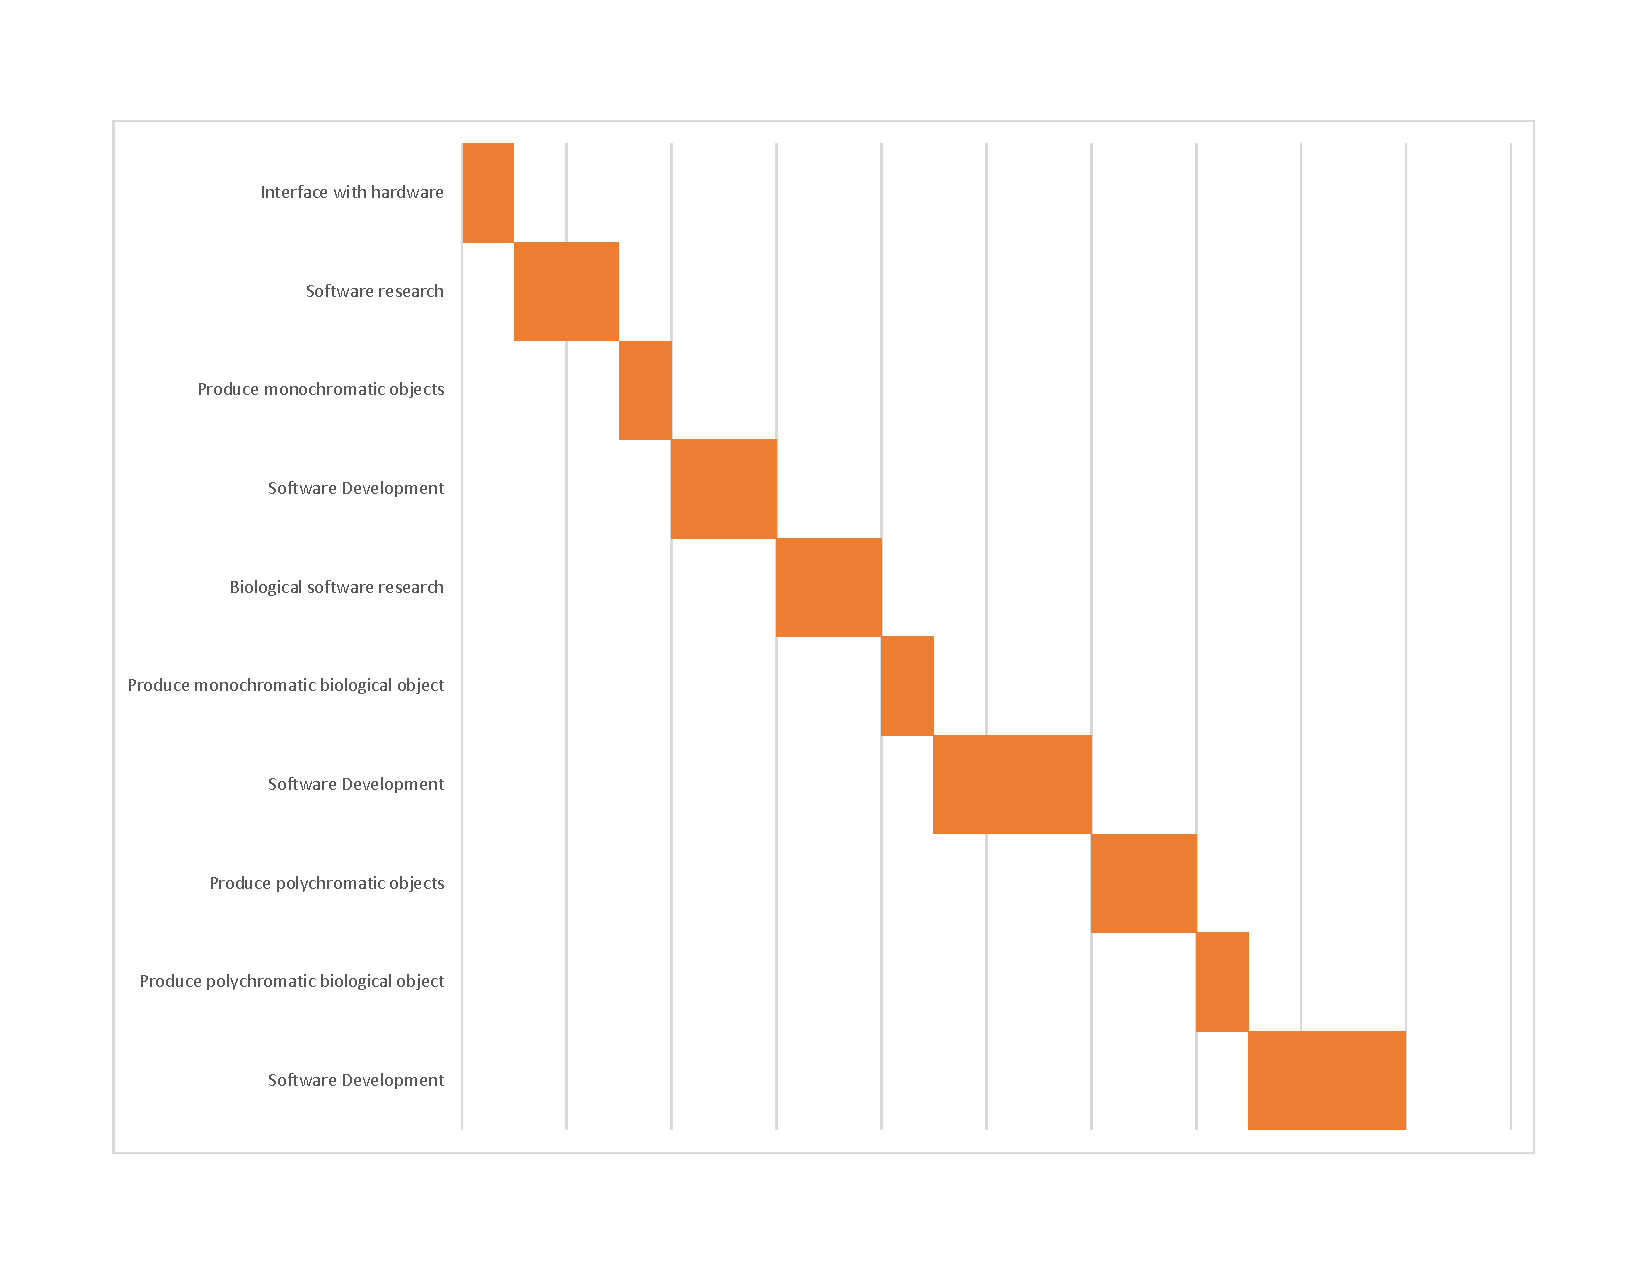
\includegraphics{gantt}
  \end{center}

\end{document}
